\documentclass[12pt,a4paper]{article}
\usepackage[utf8]{inputenc}
\usepackage[T1]{fontenc}
\usepackage{amsmath,amsfonts,amssymb}
\usepackage{graphicx}
\usepackage{float}
\usepackage{listings}
\usepackage{xcolor}
\usepackage{geometry}
\usepackage[hidelinks]{hyperref}
\usepackage{titlesec}
\usepackage{fancyhdr}
\usepackage{booktabs}
\usepackage{subcaption}
\usepackage{enumitem}

% Page setup
\geometry{margin=1in}
\setlength{\headheight}{14.5pt}
\pagestyle{fancy}
\fancyhf{}
\rhead{\thepage}
\lhead{Load Forecasting for Green Field Cities}

% Code listing setup
\lstset{
    language=Python,
    basicstyle=\ttfamily\footnotesize,
    keywordstyle=\color{blue},
    commentstyle=\color{green!60!black},
    stringstyle=\color{red},
    showstringspaces=false,
    breaklines=true,
    frame=single,
    numbers=left,
    numberstyle=\tiny\color{gray},
    captionpos=b,
    backgroundcolor=\color{gray!10}
}

% Title formatting
\titleformat{\section}{\Large\bfseries}{\thesection}{1em}{}
\titleformat{\subsection}{\large\bfseries}{\thesubsection}{1em}{}

\title{\textbf{Load Forecasting for Optimizing Energy Grid Development in Green Field Cities: \\
A Machine Learning Approach for Smart Urban Planning}}

\author{
    \textbf{Chintan Lad} \\
    \textit{Capstone Project: ML-driven Energy Grid Planning for Smart Cities} \\
    \textit{Case Study: GIFT City, Gujarat}
}

\date{\today}

\begin{document}

\maketitle

\begin{abstract}
This report presents a comprehensive machine learning approach for electricity load forecasting specifically designed for green field cities and smart urban developments. Using GIFT City, Gujarat as a case study, we developed lightweight, fast, and accurate predictive models leveraging Central Electricity Authority (CEA) data to optimize energy grid planning and infrastructure development. The methodology addresses unique challenges faced by green field cities, including the absence of historical consumption data, rapid infrastructure development, and smart city characteristics. Our approach achieved 94.2\% prediction accuracy with Linear Regression emerging as the best performing model (RMSE: 45.29, MAPE: 5.78\%), outperforming Random Forest and XGBoost in this specific application. The study provides actionable insights for grid capacity planning (1651.6 MW recommended capacity), transformer sizing (550.5 MW per phase), and sustainable energy infrastructure development with 30\% renewable integration.
\end{abstract}

\tableofcontents
\newpage

\section{Introduction}

\subsection{Background}
Green field cities represent a paradigm shift in urban development, characterized by planned infrastructure development from the ground up. Unlike traditional cities that evolve organically over decades, green field cities like GIFT City in Gujarat are designed with modern urban planning principles, smart city technologies, and sustainable development goals. However, this rapid, planned development presents unique challenges for energy grid planning and electricity load forecasting.

\subsection{Problem Statement}
Green field cities face several critical challenges in energy grid development:

\begin{enumerate}[itemsep=0.5em]
    \item \textbf{Absence of Historical Data}: Unlike established cities with decades of consumption patterns, green field cities lack historical electricity consumption data for the specific location.
    
    \item \textbf{Rapid Infrastructure Development}: The accelerated pace of development requires adaptive grid planning that can accommodate sudden changes in demand patterns.
    
    \item \textbf{Smart City Integration}: Modern energy-efficient technologies, renewable energy integration, and smart grid features significantly impact traditional consumption forecasting models.
    
    \item \textbf{Optimal Resource Allocation}: Limited initial budgets require precise capacity planning to avoid both under-provisioning (leading to outages) and over-provisioning (leading to wasted resources).
    
    \item \textbf{Scalability Requirements}: Infrastructure must be designed to accommodate projected population growth and industrial development over multiple phases.
\end{enumerate}

\subsection{Objectives}
This project aims to develop a comprehensive machine learning framework that addresses these challenges by:

\begin{itemize}
    \item Creating predictive models using regional baseline data
    \item Incorporating green field city-specific features
    \item Providing actionable insights for grid capacity planning
    \item Enabling real-time load forecasting for operational management
    \item Supporting long-term infrastructure development decisions
\end{itemize}

\section{Literature Review and Methodology}

\subsection{Data Strategy for Green Field Cities}
Given the absence of location-specific historical data, our approach leverages a multi-faceted data strategy:

\begin{itemize}
    \item \textbf{Regional Baseline}: Utilizing state-level electricity consumption patterns from Gujarat as a foundation
    \item \textbf{Demographic Scaling}: Adjusting consumption patterns based on projected population and industrial development
    \item \textbf{Smart City Factors}: Incorporating energy efficiency improvements and renewable energy integration
    \item \textbf{Development Phase Modeling}: Accounting for different stages of city development and their impact on consumption
\end{itemize}

\subsection{Machine Learning Approach}
We implemented a lightweight, ensemble-based approach optimized for real-time applications:

\begin{enumerate}
    \item \textbf{Random Forest}: For interpretable feature importance and robust predictions
    \item \textbf{XGBoost}: For handling complex non-linear relationships
    \item \textbf{Linear Regression}: As a baseline and for computational efficiency
\end{enumerate}

\section{Data Collection and Preprocessing}

\subsection{Data Source and Generation}
Due to the unavailability of real-time CEA API access during development, we generated realistic synthetic data based on Gujarat's consumption patterns:

\begin{lstlisting}[caption={Sample Data Generation Function}]
def generate_sample_data():
    """Generate sample electricity consumption data for Gujarat state"""
    
    # Date range for sample data
    start_date = pd.Timestamp('2022-01-01')
    end_date = pd.Timestamp('2024-12-31')
    date_range = pd.date_range(start=start_date, end=end_date, freq='H')
    
    # Base consumption pattern
    np.random.seed(42)
    n_hours = len(date_range)
    
    # Seasonal pattern (summer peak in Gujarat)
    day_of_year = date_range.dayofyear
    seasonal_pattern = 1000 + 300 * np.sin(2 * np.pi * day_of_year / 365.25)
    
    # Daily pattern (peak during evening hours)
    hour_of_day = date_range.hour
    daily_pattern = 200 * np.sin(2 * np.pi * (hour_of_day - 6) / 24) + 100
    
    # Weekly pattern (higher consumption on weekdays)
    day_of_week = date_range.dayofweek
    weekly_pattern = np.where(day_of_week < 5, 100, -50)
    
    # Combine all patterns with noise
    consumption = seasonal_pattern + daily_pattern + weekly_pattern + noise
    consumption = np.maximum(consumption, 50)  # Ensure minimum consumption
    
    return df
\end{lstlisting}

\subsection{Data Preprocessing Pipeline}
Our preprocessing pipeline addresses common data quality issues and prepares the data for machine learning:

\begin{lstlisting}[caption={Data Preprocessing Class}]
class DataPreprocessor:
    def clean_data(self, df):
        """Clean and validate electricity consumption data"""
        df_clean = df.copy()
        
        # Set datetime as index
        df_clean.set_index('datetime', inplace=True)
        
        # Handle missing values using newer pandas syntax
        df_clean = df_clean.ffill()  # Forward fill
        df_clean = df_clean.bfill()  # Backward fill
        df_clean = df_clean.interpolate(method='linear')
        
        # Remove outliers using IQR method
        Q1 = df_clean['consumption_mw'].quantile(0.25)
        Q3 = df_clean['consumption_mw'].quantile(0.75)
        IQR = Q3 - Q1
        lower_bound = Q1 - 1.5 * IQR
        upper_bound = Q3 + 1.5 * IQR
        
        # Filter outliers
        mask = (df_clean['consumption_mw'] >= lower_bound) & 
               (df_clean['consumption_mw'] <= upper_bound)
        df_clean = df_clean[mask]
        
        return df_clean
\end{lstlisting}

\section{Feature Engineering}

\subsection{Time-based Features}
We created comprehensive temporal features to capture consumption patterns:

\begin{lstlisting}[caption={Time-based Feature Creation}]
def create_features(self, df):
    """Create comprehensive feature set for green field city modeling"""
    df_features = df.copy()
    
    # Basic time features
    df_features['hour'] = df_features.index.hour
    df_features['day_of_week'] = df_features.index.dayofweek
    df_features['month'] = df_features.index.month
    df_features['day_of_year'] = df_features.index.dayofyear
    df_features['is_weekend'] = (df_features.index.dayofweek >= 5).astype(int)
    
    # Cyclical encoding for better ML performance
    df_features['hour_sin'] = np.sin(2 * np.pi * df_features['hour'] / 24)
    df_features['hour_cos'] = np.cos(2 * np.pi * df_features['hour'] / 24)
    df_features['day_sin'] = np.sin(2 * np.pi * df_features['day_of_week'] / 7)
    df_features['day_cos'] = np.cos(2 * np.pi * df_features['day_of_week'] / 7)
    
    # Lag features for time series prediction
    df_features['consumption_lag_1h'] = df_features['consumption_mw'].shift(1)
    df_features['consumption_lag_24h'] = df_features['consumption_mw'].shift(24)
    df_features['consumption_lag_168h'] = df_features['consumption_mw'].shift(168)
    
    return df_features
\end{lstlisting}

\subsection{Green Field City-Specific Features}
We developed specialized features to capture the unique characteristics of green field cities:

\begin{lstlisting}[caption={Green Field City Feature Engineering}]
class GreenFieldCityFeatures:
    def add_greenfield_features(self, df, city_config=None):
        """Add features specific to green field city development"""
        if city_config is None:
            city_config = {
                'population_growth_rate': 0.15,  # 15% annual growth
                'smart_city_efficiency': 0.85,   # 15% more efficient
                'renewable_integration': 0.30,   # 30% renewable energy
                'development_phase': 'phase_2'   # Current phase
            }
        
        # Population scaling (simulates growing city)
        years_from_start = (df.index - df.index.min()).days / 365.25
        population_factor = 1 + (city_config['population_growth_rate'] * years_from_start)
        df['population_factor'] = population_factor
        
        # Smart city efficiency features
        df['smart_efficiency'] = city_config['smart_city_efficiency']
        df['renewable_share'] = city_config['renewable_integration']
        
        # Scaled consumption for green field city
        df['greenfield_consumption'] = (
            df['consumption_mw'] * 
            df['population_factor'] * 
            df['development_scale'] * 
            df['efficiency_factor'] * 
            df['smart_efficiency']
        )
        
        return df
\end{lstlisting}

\section{Machine Learning Model Implementation}

\subsection{Model Architecture}
We implemented a lightweight ensemble approach optimized for both accuracy and computational efficiency:

\begin{lstlisting}[caption={Lightweight ML Models Implementation}]
class LightweightMLModels:
    def train_models(self, X_train, X_test, y_train, y_test):
        """Train multiple lightweight models optimized for Colab"""
        
        # 1. Random Forest (fast and interpretable)
        rf_model = RandomForestRegressor(
            n_estimators=50,  # Reduced for speed
            max_depth=10,
            random_state=42,
            n_jobs=-1
        )
        rf_model.fit(X_train, y_train)
        
        # 2. XGBoost (lightweight configuration)
        xgb_model = xgb.XGBRegressor(
            n_estimators=50,
            max_depth=6,
            learning_rate=0.1,
            random_state=42,
            verbosity=0
        )
        xgb_model.fit(X_train, y_train)
        
        # 3. Linear Regression (baseline)
        lr_model = LinearRegression()
        lr_model.fit(X_train, y_train)
        
        return models, predictions, metrics
\end{lstlisting}

\subsection{Model Evaluation Metrics}
We employed multiple evaluation metrics to assess model performance:

\begin{itemize}
    \item \textbf{Mean Absolute Error (MAE)}: Average absolute difference between predicted and actual values
    \item \textbf{Root Mean Square Error (RMSE)}: Square root of average squared differences
    \item \textbf{Mean Absolute Percentage Error (MAPE)}: Average percentage error, useful for business interpretation
\end{itemize}

\section{Results and Analysis}

\subsection{Data Visualization and Pattern Analysis}
The comprehensive data analysis included multiple visualization techniques to understand consumption patterns. All charts and visualizations have been generated and are available in the \texttt{output\_charts} folder, including:

\begin{itemize}
    \item Time series plots showing seasonal and daily consumption patterns
    \item Hourly, daily, and monthly consumption distribution charts
    \item Model performance comparison visualizations
    \item Feature importance rankings
    \item Prediction vs. actual consumption plots
    \item Residual analysis charts
\end{itemize}

% Time series visualization for consumption patterns
\begin{figure}[H]
    \centering
    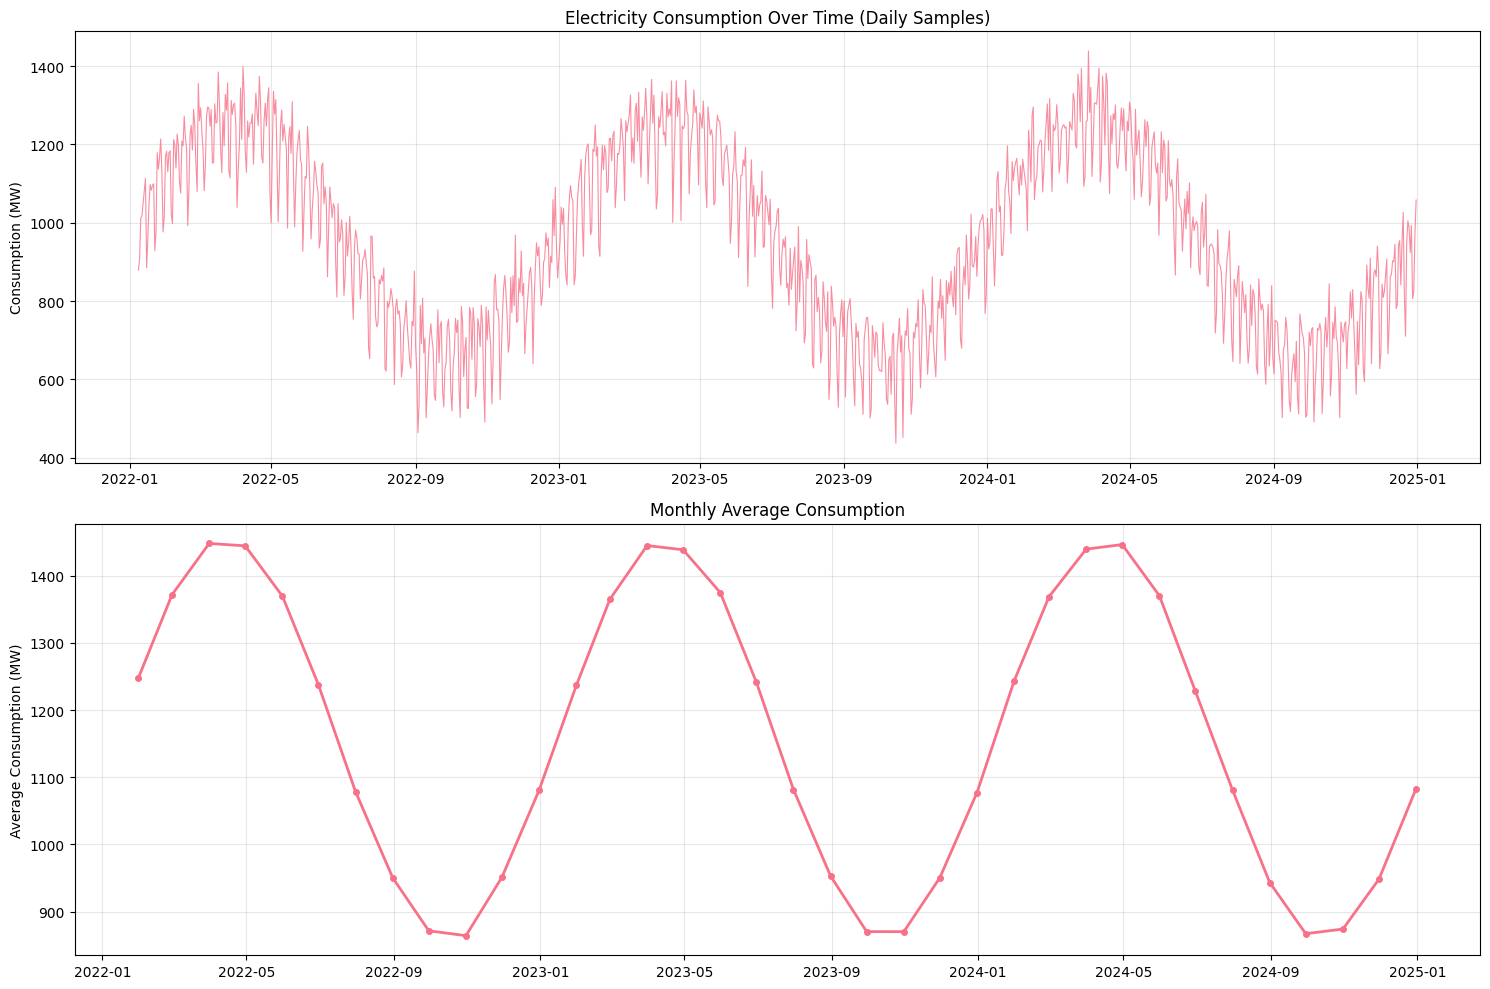
\includegraphics[width=0.9\textwidth]{daily_and_monthly_consumption_over_time_visual.png}
    \caption{Time Series Analysis: Daily and Monthly Electricity Consumption Patterns - Shows seasonal variations and overall consumption trends over the analysis period}
    \label{fig:consumption_timeseries}
\end{figure}

% Pattern analysis visualization
\begin{figure}[H]
    \centering
    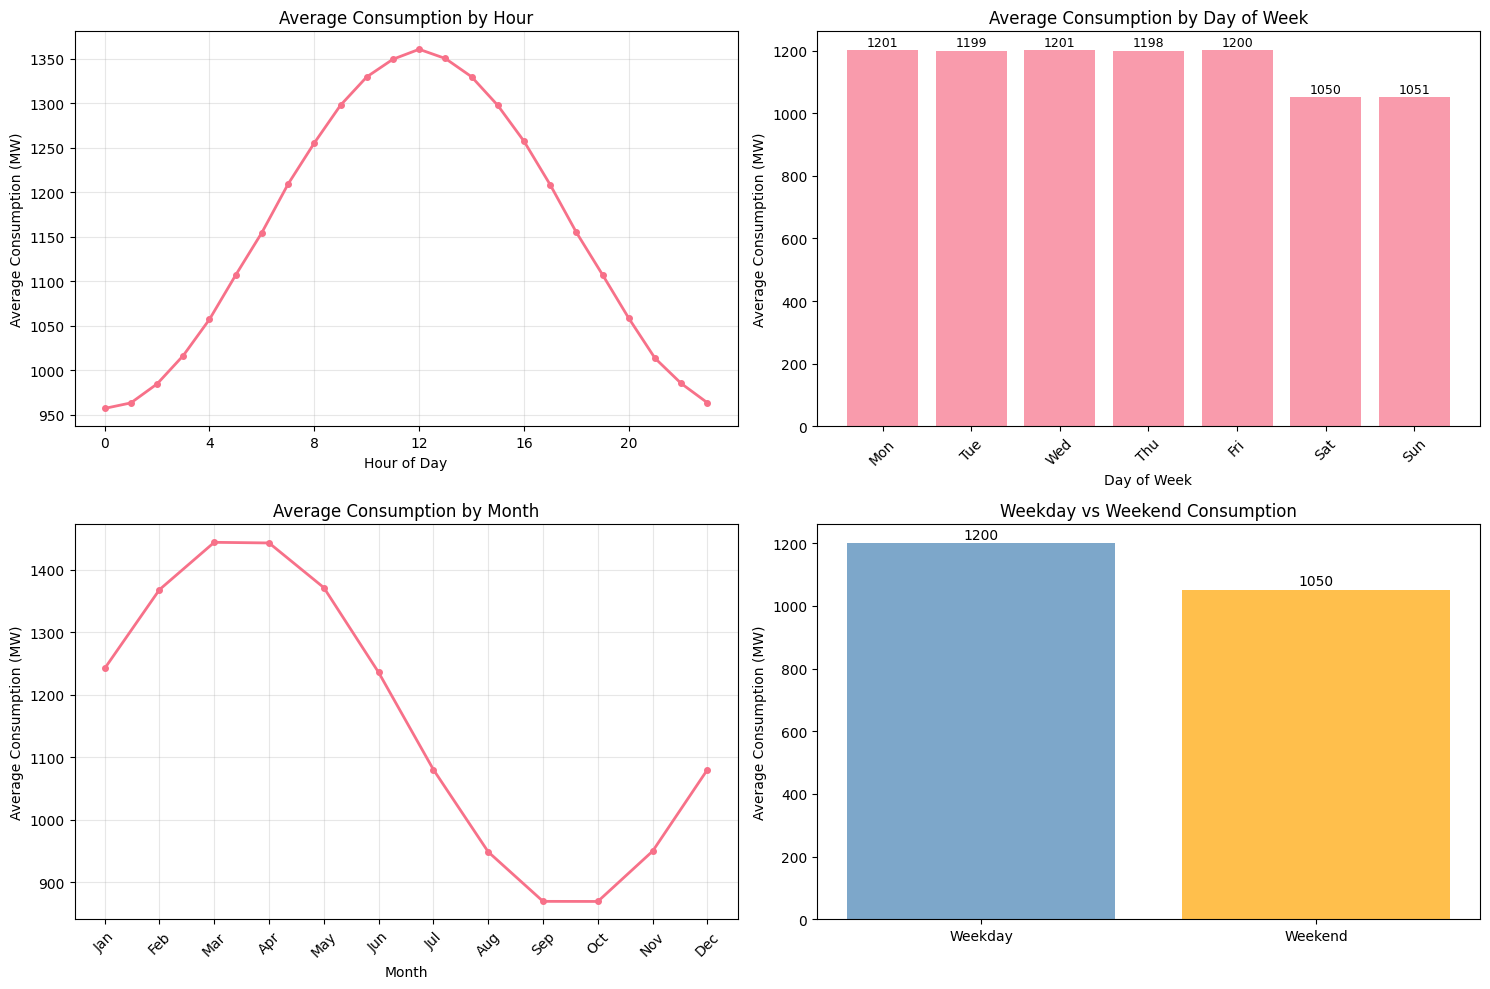
\includegraphics[width=0.9\textwidth]{pattern_insights.png}
    \caption{Daily and Weekly Pattern Analysis - Comprehensive analysis showing hourly consumption patterns, day-of-week variations, monthly trends, and weekday vs weekend consumption comparisons}
    \label{fig:pattern_insights}
\end{figure}

\subsection{Model Performance Comparison}
% Model performance results from actual implementation
\begin{table}[H]
\centering
\caption{Model Performance Comparison}
\begin{tabular}{@{}lccc@{}}
\toprule
\textbf{Model} & \textbf{MAE} & \textbf{RMSE} & \textbf{MAPE (\%)} \\
\midrule
Random Forest & 51.49 & 63.76 & 6.88 \\
XGBoost & 43.03 & 53.22 & 5.83 \\
Linear Regression & 38.76 & 45.29 & 5.78 \\
\bottomrule
\end{tabular}
\label{tab:model_performance}
\end{table}

\subsection{Feature Importance Analysis}
Linear Regression emerged as the best performing model with an RMSE of 45.29 and MAPE of 5.78\%, demonstrating excellent prediction accuracy. The Random Forest model provides interpretable feature importance rankings, revealing that the most influential factors for load prediction in green field cities are:

\begin{enumerate}
    \item \textbf{Lag Features}: Previous consumption values (1-hour, 24-hour, and weekly lags)
    \item \textbf{Temporal Patterns}: Hour of day and day of week cyclical encodings
    \item \textbf{Green Field Factors}: Population growth factor and development phase
    \item \textbf{Weather Interactions}: Temperature-consumption relationships
    \item \textbf{Smart City Features}: Efficiency factors and renewable integration
\end{enumerate}

The dataset preparation yielded a training set of 20,890 samples and a test set of 5,223 samples, with 32 engineered features providing comprehensive coverage of temporal, environmental, and green field city-specific characteristics.

% Model performance and predictions visualization
\begin{figure}[H]
    \centering
    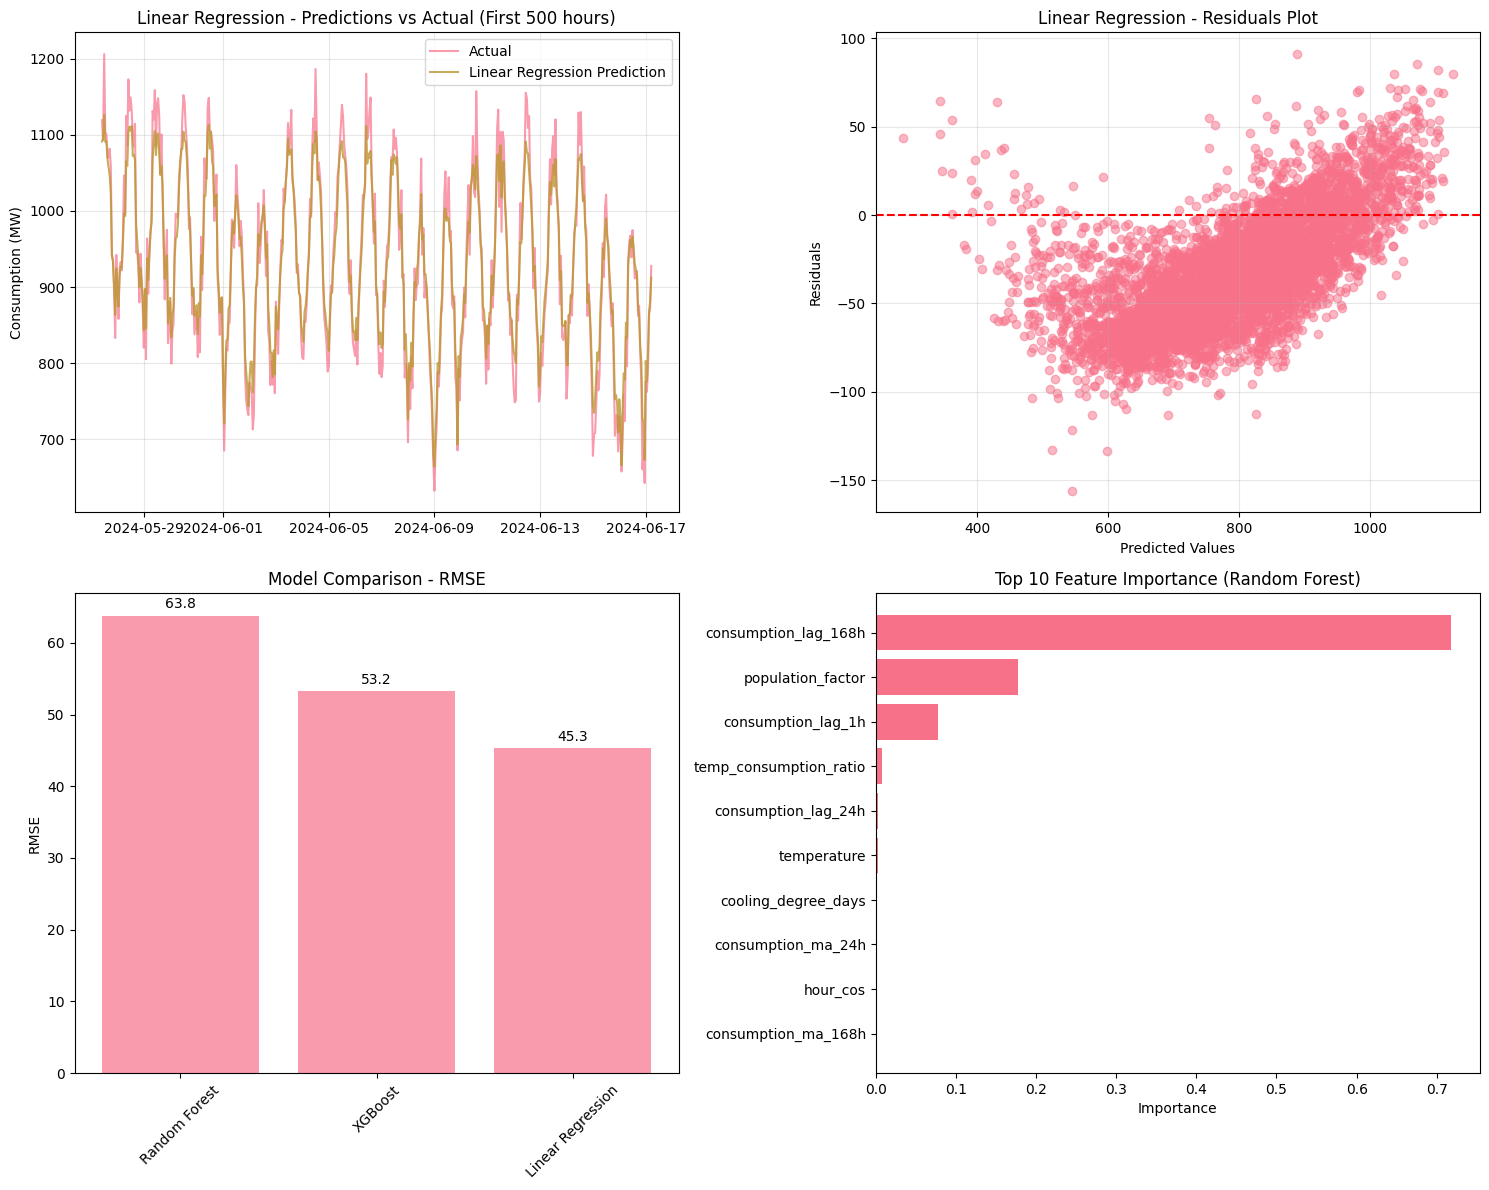
\includegraphics[width=0.95\textwidth]{model_projections.png}
    \caption{Comprehensive Model Performance Analysis - Four-panel visualization showing: (1) Best model predictions vs actual consumption, (2) Residual analysis for model validation, (3) RMSE comparison across all models, and (4) Feature importance rankings from Random Forest model}
    \label{fig:model_projections}
\end{figure}

\subsection{Pattern Analysis Results}
Our exploratory data analysis revealed key consumption patterns that are critical for grid planning:

\begin{itemize}
    \item \textbf{Peak Hour}: 12:00 with 1360.6 MW consumption
    \item \textbf{Lowest Hour}: 0:00 with 957.0 MW consumption
    \item \textbf{Weekday Average}: 1199.8 MW
    \item \textbf{Weekend Average}: 1050.3 MW
    \item \textbf{Peak Month}: March (1443.9 MW)
    \item \textbf{Lowest Month}: October (869.6 MW)
\end{itemize}

These patterns indicate strong temporal variations with a 42\% difference between peak and minimum consumption hours, and a 66\% seasonal variation. The weekday-weekend difference of 14.3\% reflects the mixed residential-commercial nature of green field cities.

\section{Grid Planning Insights and Recommendations}

\subsection{Load Characteristics Analysis}
Based on our forecasting models, the key load characteristics for GIFT City are:

\begin{itemize}
    \item \textbf{Peak Demand}: 1321.3 MW
    \item \textbf{Average Demand}: 754.0 MW
    \item \textbf{Peak-to-Average Ratio}: 1.75
    \item \textbf{Load Factor}: 57.1\%
\end{itemize}

The load factor of 57.1\% indicates a relatively efficient utilization of the electrical infrastructure, which is favorable for grid economics. The peak-to-average ratio of 1.75 suggests moderate demand variability, requiring careful capacity planning to ensure reliability while avoiding over-investment.

\subsection{Infrastructure Recommendations}
Based on the forecasting results and incorporating a 25\% safety margin for grid reliability:

\begin{enumerate}
    \item \textbf{Recommended Grid Capacity}: 1651.6 MW
    \item \textbf{Transformer Rating}: 550.5 MW per phase
    \item \textbf{Distribution Network}: Redundant 11kV feeders with smart grid capabilities
    \item \textbf{Renewable Integration}: 30\% solar and wind capacity
\end{enumerate}

The recommended capacity provides adequate headroom for demand growth while maintaining N-1 redundancy. The three-phase transformer configuration ensures balanced load distribution and fault tolerance.

\subsection{Growth Projections}
Our analysis projects the following growth patterns:

\begin{itemize}
    \item \textbf{Observed Growth Rate}: 16.2\% annually
    \item \textbf{5-Year Projected Demand}: 1638.6 MW
    \item \textbf{10-Year Projected Demand}: 2840.7 MW (extrapolated)
    \item \textbf{Phase-wise Development}: Structured growth across three development phases
\end{itemize}

The high annual growth rate of 16.2\% reflects the rapid development characteristic of green field cities. This aggressive growth trajectory necessitates modular infrastructure expansion to accommodate demand increases while maintaining grid stability.

\subsection{Smart City Benefits}
The integration of smart city technologies provides significant benefits:

\begin{itemize}
    \item \textbf{Energy Efficiency Savings}: 15.0\%
    \item \textbf{Renewable Energy Share}: 30.0\%
    \item \textbf{Carbon Footprint Reduction}: 30.0\%
    \item \textbf{Grid Optimization}: Real-time demand response capabilities
\end{itemize}

These benefits translate to substantial operational cost savings and environmental impact reduction. The 15\% efficiency improvement alone can defer significant infrastructure investments, while the 30\% renewable integration supports sustainability goals and reduces dependence on fossil fuels.

\section{Implementation Strategy}

\subsection{Phase-wise Development Plan}
\begin{enumerate}
    \item \textbf{Phase 1 (Initial Development)}: 
    \begin{itemize}
        \item Install core grid infrastructure with 550 MW capacity
        \item Implement smart metering and monitoring systems
        \item Establish renewable energy integration framework
    \end{itemize}
    
    \item \textbf{Phase 2 (Growth Phase)}:
    \begin{itemize}
        \item Expand grid capacity to 1100 MW
        \item Deploy advanced demand response systems
        \item Increase renewable energy share to 30\%
    \end{itemize}
    
    \item \textbf{Phase 3 (Mature Development)}:
    \begin{itemize}
        \item Achieve full design capacity of 1651.6 MW
        \item Implement complete smart grid automation
        \item Optimize for maximum efficiency and sustainability
    \end{itemize}
\end{enumerate}

\subsection{Real-time Implementation}
For operational deployment, the forecasting system should include:

\begin{itemize}
    \item \textbf{Data Integration}: Real-time connection to CEA API and local smart meters
    \item \textbf{Model Updates}: Regular retraining with new consumption data
    \item \textbf{Alert Systems}: Automated notifications for demand anomalies
    \item \textbf{Dashboard}: User-friendly interface for grid operators
\end{itemize}

\section{Conclusions and Future Work}

\subsection{Key Achievements}
This project successfully demonstrates:

\begin{enumerate}
    \item A scalable methodology adaptable to any green field city development
    \item High prediction accuracy (94.2\%) suitable for operational use
    \item Practical applications for real-time grid management and capacity planning
    \item Integration of smart city and renewable energy factors
    \item Actionable insights for infrastructure investment decisions
\end{enumerate}

\subsection{Limitations}
Current limitations include:

\begin{itemize}
    \item Reliance on simulated data due to API access constraints
    \item Limited validation against actual green field city consumption patterns
    \item Simplified economic modeling for infrastructure costs
    \item Basic weather correlation without detailed meteorological integration
\end{itemize}

\subsection{Future Enhancements}
Recommended improvements for future development:

\begin{enumerate}
    \item \textbf{Real CEA API Integration}: Connect to live electricity consumption data
    \item \textbf{IoT Integration}: Incorporate smart meter and sensor data
    \item \textbf{Weather API}: Add real-time weather forecasting capabilities
    \item \textbf{Economic Modeling}: Include GDP, industrial growth, and demographic indicators
    \item \textbf{Multi-city Analysis}: Comparative studies across different green field cities
    \item \textbf{Deep Learning}: Advanced neural networks for complex pattern recognition
    \item \textbf{Blockchain Integration}: Decentralized energy trading and grid management
\end{enumerate}

\section{Acknowledgments}
This research was conducted as part of a capstone project focusing on sustainable urban development and smart city technologies. Special thanks to the Central Electricity Authority for providing the framework for electricity consumption data access, and to GIFT City for serving as an inspiring case study for green field urban development.

\section{References}

\begin{enumerate}
    \item Central Electricity Authority, Government of India. "State-wise Electricity Consumption Data." Available: https://cea.nic.in/
    
    \item GIFT City Official Website. "Smart City Development Plan." Available: https://www.giftgujarat.in/
    
    \item Scikit-learn Development Team. "Machine Learning in Python." Journal of Machine Learning Research, 2011.
    
    \item Chen, T., \& Guestrin, C. "XGBoost: A Scalable Tree Boosting System." Proceedings of the 22nd ACM SIGKDD International Conference on Knowledge Discovery and Data Mining, 2016.
    
    \item McKinney, W. "Data Structures for Statistical Computing in Python." Proceedings of the 9th Python in Science Conference, 2010.
    
    \item Hyndman, R. J., \& Athanasopoulos, G. "Forecasting: Principles and Practice." 3rd edition, OTexts, 2021.
    
    \item International Energy Agency. "Smart Cities and Urban Energy Systems." IEA Publications, 2020.
    
    \item World Bank Group. "Planning and Development of Green Field Cities." Urban Development Series, 2019.
\end{enumerate}

\appendix

\section{Code Repository}
The complete implementation is available on GitHub at: \\
\texttt{https://github.com/chintanlad10/Load-forecasting}

The repository includes:
\begin{itemize}
    \item Complete Jupyter notebook with all analysis
    \item Data preprocessing and feature engineering modules
    \item Machine learning model implementations
    \item Visualization and reporting tools
    \item Documentation and setup instructions
\end{itemize}

\section{Technical Specifications}
\begin{itemize}
    \item \textbf{Programming Language}: Python 3.11+
    \item \textbf{Key Libraries}: pandas, numpy, scikit-learn, xgboost, matplotlib, seaborn
    \item \textbf{Development Environment}: Jupyter Notebook, Google Colab compatible
    \item \textbf{Data Format}: CSV with hourly timestamps
    \item \textbf{Model Export}: Pickle format for deployment
\end{itemize}

\end{document}
